\documentclass{standalone}
\usepackage{pgfplots}
\usepackage{mhchem}
\pgfplotsset{compat=1.18}

\begin{document}
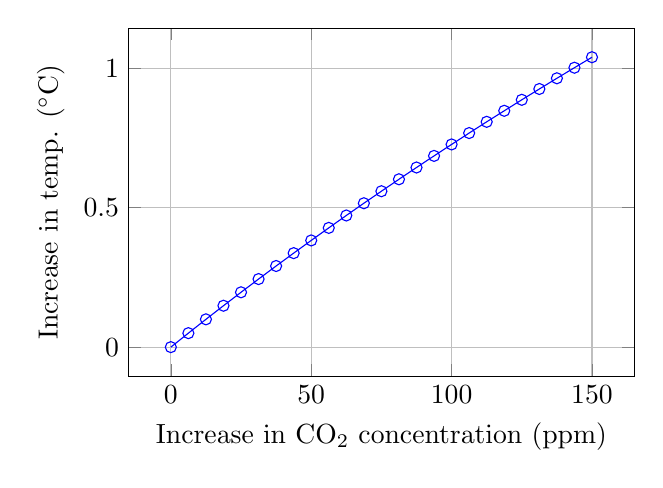
\begin{tikzpicture}
	\begin{axis}[
		xlabel={Increase in \ce{CO2} concentration (ppm)},
		ylabel={Increase in temp. ($\rm ^\circ C$)},
		width=8cm, height=6cm,
		grid=major
	]
		\addplot[domain=0:150, mark=o, blue] {3.42 * ln((422 + x) / 422)};
	\end{axis}
\end{tikzpicture}
\end{document}